% Chapter Template

\chapter{Results} % Main chapter title

\label{Chapter5} % Change X to a consecutive number; for referencing this chapter elsewhere, use \ref{ChapterX}

%----------------------------------------------------------------------------------------
%	SECTION 1
%----------------------------------------------------------------------------------------

\section{Balance Sheet Ratios}

The average observed liquidity ratios shown in Figure \ref{fig:Ratios} for all companies of the dataset are showing an increase in liquidity in 2020 and 2021 compared to the pre pandemic years indication that companies are holding relatively more cash at the year-end since the pandemic. A study conducted by the German Federal Bank reported an increase in the average cash ratio for German companies in 2020 as well as in 2021 \parencite{deutsche_bundesbank_jahresabschlussstatistik_2022}. For example, for SME corporations the study reported a change in the cash ratio from 0.104 (2019) to 0.110 (2020). For the current ratio and quick ratio, the same trend was reported. Further support for an increase in the quick ratio was found by another study \parencite{bley_mittelstand_2022}. Although the exact ratios are varying between studies, there is strong support for the general trend of increasing liquidity in 2020 and 2021.

Solvency ratios are showing a less clear trend after the COVID-19 pandemic. Although minimal, the opposite trends in the equity ratio and debt-to-asset-ratio are as expected. The only visible change happened in 2020, while in 2021 the ratios are very similar to 2018 and 2019. The change in the debt-to-asset ratio is amplified in the debt-to-equity ratio, as expected. Survy Data from the KFW found an Equity Ratio of 0.318 in 2019, a decrease to 0.301 in 2020 and a recovery to 0.314 in 2021 \parencite{kfw_kfw-mittelstandspanel_2022}. For very small companies with less than 10 employees, the drop in 2020 was stronger, and the recovery in 2021 was above pre-pandemic levels. Lager companies did not have a recovery after the crisis year and decreased their Equity Ratio in 2021 on average further. This could indicate that the recovery of the indebtedness in 2021 might have been driven by smaller companies. Similar observations were reported by the German Federal Bank were the debt-to-asset-ratio for SME corporations decreased in 2020.


\begin{figure}
\centering
\makebox[\textwidth][c]{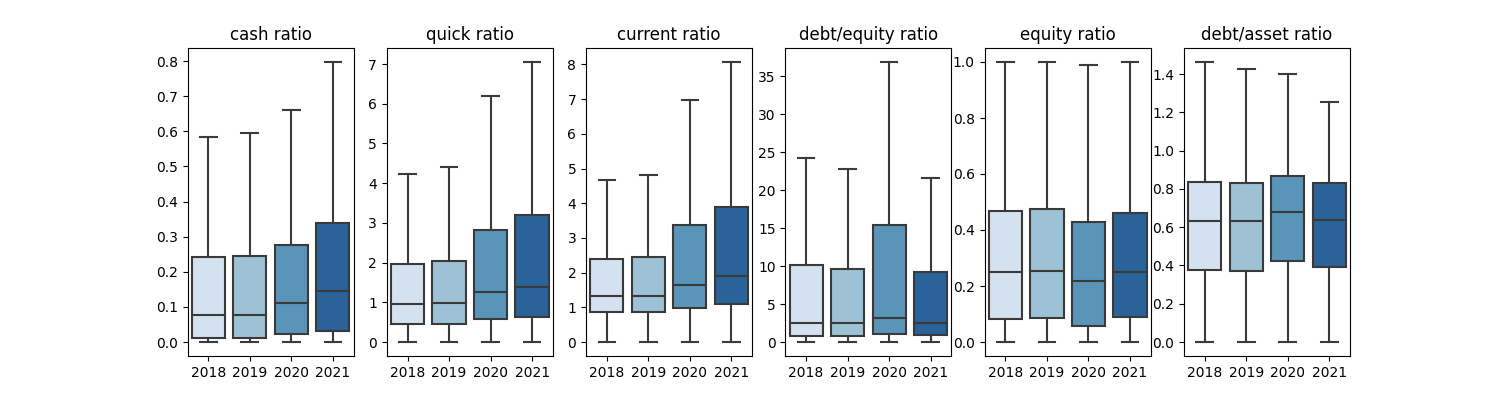
\includegraphics[width=1.2\columnwidth]{Figures/chart_ratios}}%

\decoRule
\caption[Balance sheet ratios]{Boxplot with balance sheet ratios from the obained dataset.}
\label{fig:Ratios}
\end{figure}


%----------------------------------------------------------------------------------------
%	SECTION 2
%----------------------------------------------------------------------------------------

\section{Difference-in-Differences}

The interaction terms from the difference-in-differences regressions are shown in table \ref{tab:DiDresults}. The coefficients for the aid and post are reported in Appendix \ref{AppendixA}. In the first-row cash ratio coefficients are reported for grants and loans. In the 2020 column the effect for grants is the only cash ratio coefficient that is not statistically significant. In 2021 the coefficient for grants on the cash ratio was estimated to be 7.68 \% indicating a strong causal effect. The average treatment effect for firms that got aid through loans is positive in 2020 and 2021, but less strong than grants. Also, the effect in 2021 is less strong compared to 2021.

The quick ratio and the current ratio only have statistically significant for loans. At a significance level of 1 \% only the quick ratio and the current ratio coefficient for 2020 are significant. The treatment effects with 10.85 \% and 12.71 \% are even stronger than for that cash ratio. The effects for current ratio are even larger, reflecting the proportionality between the ratios. Overall, the results show strong effects of loan on the observed liquidity ratios. For grants an even stronger effect was observed in 2021, but only for the cash ratio, not for the more conservative ratios. This could be caused by the alternative the calculation that was used for part of the companies. 

In the row for the debt-to-equity ratio strongly positive coefficients were observed for loans in 2020 and 2021. Since the debt-to-equity ratio reflects a firm’s leverage it is plausible that loans have a causal effect on debt. Regarding the equity ratio in following row a negative effect of loans was estimated for 2020 and 2021. For grants, which aren’t affecting a firm’s debt, no statistically significant effect was observable and thus indicating that grants didn’t support the equity of firm. Further support for the increase in leverage through loans comes from the debt-to-asset ratio coefficients. The effects for loans are strong in 2020 and 2021 with 7.15 \% and 5.26 \%. 
For grants the causal effect is 4,12 \% in 2020 and reversing in 2021 to - 3.02 \%. The positive effect in 2020 is in line with missing effect on the equity ratio. The negative coefficient in 2021 on the other hand, indicates that grants helped firm’s to reduce leverage by slightly.
In summary both aid measures have a significant effect on the cash ratio indicating a liquidity boost. This indicates that loans were not used for refinancing, but actually served as liquidity injection as intended by the policy makers. Also, the increase in leverage from loans is measurable as expected. However, the estimates doesn`t support the expectation that grant protect the equity. The positive effect of grants on debt-to-asset ratio and the missing effect on the cash ratio in 2020 suggests that the aid was not sufficient for the liquidity short falls and companies had to rely on debt from other sources for liquidity injections. The reversal in 2021 suggests that grants only became effective in 2021. However, this could be related to the fact that only relatively little grants were provided in 2020.


\begin{table}
    \caption{Government aid impact on ratios}
    \label{tab:DiDresults}
    \centering
    \def\arraystretch{1.5}
    \centering
    \begin{tabular}{llrr}
\toprule
                     & \textbf{year} &                                    2020 &                                    2021 \\
{} & \textbf{instrument} &                                         &                                         \\
\midrule
\multirow{2}{*}{\textbf{cash ratio}} & \textbf{grant} &  -0.0089\space\space\space\space(0.270) &                  0.0768***\space(0.000) \\
                     & \textbf{loan} &                  0.0527***\space(0.000) &                  0.0351***\space(0.000) \\
\cline{1-4}
\multirow{2}{*}{\textbf{quick ratio}} & \textbf{grant} &  -0.0937\space\space\space\space(0.221) &   0.0913\space\space\space\space(0.478) \\
                     & \textbf{loan} &                  0.1085***\space(0.000) &   0.0929\space\space\space\space(0.252) \\
\cline{1-4}
\multirow{2}{*}{\textbf{current ratio}} & \textbf{grant} &  -0.0825\space\space\space\space(0.330) &   0.0476\space\space\space\space(0.736) \\
                     & \textbf{loan} &                  0.1271***\space(0.000) &        0.1828*\space\space\space(0.064) \\
\cline{1-4}
\multirow{2}{*}{\textbf{debt to equity ratio}} & \textbf{grant} &        0.2478*\space\space\space(0.089) &  -0.1592\space\space\space\space(0.185) \\
                     & \textbf{loan} &                  0.7306***\space(0.000) &             0.5043**\space\space(0.016) \\
\cline{1-4}
\multirow{2}{*}{\textbf{equity ratio}} & \textbf{grant} &  -0.0112\space\space\space\space(0.371) &   0.0108\space\space\space\space(0.465) \\
                     & \textbf{loan} &                 -0.0486***\space(0.000) &                  -0.037***\space(0.004) \\
\cline{1-4}
\multirow{2}{*}{\textbf{debt to assest ratio}} & \textbf{grant} &                  0.0412***\space(0.006) &       -0.0302*\space\space\space(0.079) \\
                     & \textbf{loan} &                  0.0715***\space(0.000) &                  0.0526***\space(0.002) \\
\bottomrule
\end{tabular}
}

    \small  Notes: Standard errors in parentheses, *** p<0.01, ** p<0.05, * p<0.1

    \end{table}


%----------------------------------------------------------------------------------------
%	SECTION 3
%----------------------------------------------------------------------------------------

\section{Causal Curve}

